\documentclass[a4paper,12pt]{article}
\usepackage[utf8]{inputenc}
\usepackage[T1]{fontenc}
\usepackage[serbian]{babel}
\usepackage{amsmath}
\usepackage{graphicx}
\usepackage{geometry}
\geometry{margin=1in}
\title{Klasifikacija zvezda od galaksija korišćenjem klasifikacionih algoritama}
\author{\\Aleksa Toroman 84/2018 & Milica Sudar 79/2017 \\\\ Univerzitet u Beogradu, Matematički fakultet}

\begin{document}

\maketitle

\newpage
\renewcommand{\contentsname}{Sadržaj}
\tableofcontents

\newpage

\section{Uvod}
Klasifikacija nebeskih objekata na zvezde i galaksije predstavlja jedan od ključnih izazova u astronomiji i astrofizici. Tačna klasifikacija ovih objekata omogućava bolje razumevanje strukture i evolucije svemira. U ovom radu istražujemo primenu različitih klasifikacionih algoritama za predikciju da li je nebeski objekat zvezda ili galaksija na osnovu dostupnih podataka.\\
Cilj ovog istraživanja je da se primenom različitih klasifikacionih algoritama postigne visoka tačnost u klasifikaciji, kao i da se identifikuju ključni atributi koji najviše doprinose tačnosti predikcija. Kroz rad ćemo se osvrnuti na metodologiju korišćenu u analizi, opis podataka, implementaciju algoritama, analizu rezultata i zaključke do kojih smo došli.

\section{Metodologija}
\subsection{Softverski alati i okruženje}
Za potrebe ovog istraživanja korišćeni su sledeći softverski alati i okruženja:
\begin{itemize}
    \item \textbf{PyCharm}: Integrisano razvojno okruženje (IDE) za Python, koje omogućava efikasno kodiranje, debugovanje i testiranje.
    \item \textbf{Python}: Glavni programski jezik korišćen za implementaciju algoritama, analizu podataka i vizualizaciju rezultata.
    \item \textbf{Jupyter Notebook}: Interaktivno okruženje za analizu podataka i vizualizaciju, koje omogućava lako eksperimentisanje sa kodom i pregled rezultata.
\end{itemize}

\subsection{Korišćene biblioteke}
Za analizu podataka i implementaciju klasifikacionih algoritama korišćene su sledeće Python biblioteke:
\begin{itemize}
    \item \textbf{pandas}: Za manipulaciju i analizu podataka.
    \item \textbf{numpy}: Za numeričke operacije i rad sa nizovima.
    \item \textbf{scikit-learn}: Za implementaciju i evaluaciju klasifikacionih algoritama.
    \item \textbf{matplotlib} i \textbf{seaborn}: Za vizualizaciju podataka i rezultata.
\end{itemize}


\section{Podaci i Pretprocesiranje}
U ovom istraživanju razmatrana su dva različita skupa podataka: jedan sa SuperCOSMOS Sky Survey sajta i drugi sa Sloan Digital Sky Survey sajta. U nastavku ćemo opisati način prikupljanja, učitavanja i pretprocesiranja podataka za oba skupa.

\subsection{SuperCOSMOS Sky Survey}
Podaci sa SuperCOSMOS Sky Survey sajta prikupljeni su korišćenjem dostupnih pretraga i alata za ekstrakciju podataka dostupnih na zvanicnom sajtu. Originalno, skup podataka je sadržao 901,322 redova i 43 atributa, međutim deo atributa koji je bio bitan za proces klasifikacije je imao određene nedostatke.

Tokom pretprocesiranja podataka identifikovano je nekoliko značajnih problema:
\begin{itemize}
    \item \textbf{Magnituda}: Mnoge vrednosti za magnitude (u, g, r, i, z) su bile prazne ili su imale placeholder vrednosti koje su bile velike cifre, što je indiciralo nedostatak stvarnih podataka ili prisustvo grešaka. Ove vrednosti su morale biti odstranjene pre dalje analize.
    \item \textbf{RA i DEC}: Vrednosti za Celestial Right Ascension (RA) i Celestial Declination (DEC) su bile vrlo slične za sve redove, što je ukazivalo na to da su podaci dobijeni sa ograničenog područja neba. Ovo je bilo posledica limitacije upita  koji je vraćao podatke samo iz određenih regiona sa definisanim radijusom pretrage.
\end{itemize}

Nakon uklanjanja nedostajućih vrednosti i outlier-a, preostalo je svega 80,000 redova za dalju analizu, što je znatno manje od originalnih 1,000,000 redova. Ovo smanjenje broja redova je posledica visokog procenta nedostajućih vrednosti i prisustva placeholder-a koji su značajno umanjili kvalitet podataka.

\subsection{Sloan Digital Sky Survey}
Podaci sa Sloan Digital Sky Survey (SDSS) sajta prikupljeni su korišćenjem odgovarajućeg SQL upita na njihovom data centru. Upit je konstruisan kako bi se dohvatili svi potencijalno relevantni atributi za vizualizaciju i treniranje klasifikacionog modela.

\begin{figure}[h!]
\centering
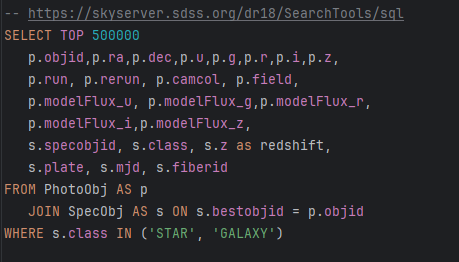
\includegraphics[width=0.8\textwidth]{sql.png}
\caption{SQL upit korišćen za prikupljanje podataka sa SDSS sajta}
\label{fig:sql_query}
\end{figure}

Ovim upitom dohvaćeno je 500,000 redova, obuhvatajući sve potencijalno bitne atribute za dalju analizu. Spektar atributa koji je dostupan putem SDSS baze podataka je značajno veći u odnosu na SuperCOSMOS, što omogućava bogatiju analizu i bolje treniranje modela. Istraživanjem šeme podataka u SDSS bazi, identifikovan je veći broj atributa koji mogu biti korisni za klasifikaciju.\\\\
S obzirom na to da je klasifikacija u ovom istraživanju fokusirana na razlikovanje zvezda i galaksija, eksplicitno smo tražili da se dohvate podaci koji uključuju samo one klase objekata koje pripadaju ili zvezdama ili galaksijama, isključujući quasare kao tip nebeskih objekata.\\\\
Pretprocesiranje podataka sa SDSS sajta pokazalo je znatno manji broj nedostajućih vrednosti i outlier-a u poređenju sa SuperCOSMOS Sky Survey skupom podataka. Nakon čišćenja podataka, preostalo je oko 492,000 redova koji su bili kvalitetni za dalju analizu. S obzirom na viši kvalitet podataka kao i veći broj slogova, dalji rad i analiza u ovom istraživanju fokusirani su na ovaj skup podataka.

\subsection{Učitavanje i čišćenje podataka}


\subsubsection{Učitavanje podataka}
Podaci su učitani korišćenjem biblioteke pandas, koja je moćan alat za manipulaciju i analizu podataka u Pythonu. Nakon učitavanja, proverili smo da li je skup podataka uspešno dovučen i uradili smo osnovne operacije za pregled podataka i njegove statistike. Takođe u ovom procesu su i isključene kolone koje nisu potrebne za dalju analizu i treniranje modela za klasifikaciju (više o ovome u narednoj sekciji):

\begin{figure}[h!]
\centering
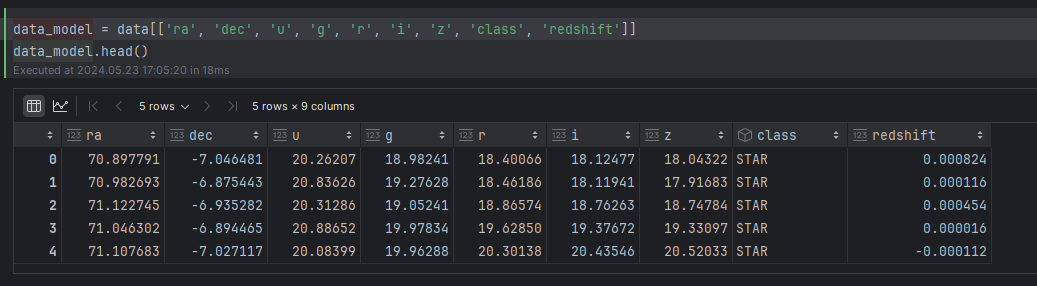
\includegraphics[width=0.8\textwidth]{list_data.png}
\caption{Izlistavanje nekolicine redova učitanog skupa podataka}
\label{fig:sql_query}
\end{figure}

\clearpage

\subsubsection{Identifikacija i uklanjanje anomalija}
Proces čišćenja podataka je ključan korak u pripremi podataka za treniranje modela. Ovaj proces uključuje identifikaciju i uklanjanje anomalija i outlier-a i razrešavanje praznih vrednosti.\\\\
Prvo smo proverili da li skup podatak ima nedostajuće vrednosti u nekim kolonama:

\begin{figure}[h!]
\centering
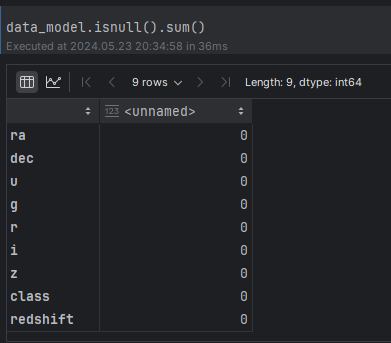
\includegraphics[width=0.8\textwidth]{null_column_check.png}
\caption{Provera nedostajućih vrednosti u kolonama}
\label{fig:sql_query}
\end{figure}

Međutim, naš skup podataka nije imao takav slučaj pa smo obradu ovakvih redova preskočili.

\clearpage
Za uklanjanje outlier-a koristili smo algoritam Local Outlier Factor (LOF) za identifikaciju i uklanjanje outlier-a. LOF algoritam procenjuje udaljenost svakog podatka od njegovih suseda i identifikuje one podatke koji se značajno razlikuju od ostatka skupa.\\\\
Takođe, i bez algoritma jednostavnim pregledom osnovih statistika smo uvideli da neke kolone u sebi imaju određene anomalije:\\\\

\begin{figure}[h!]
\centering
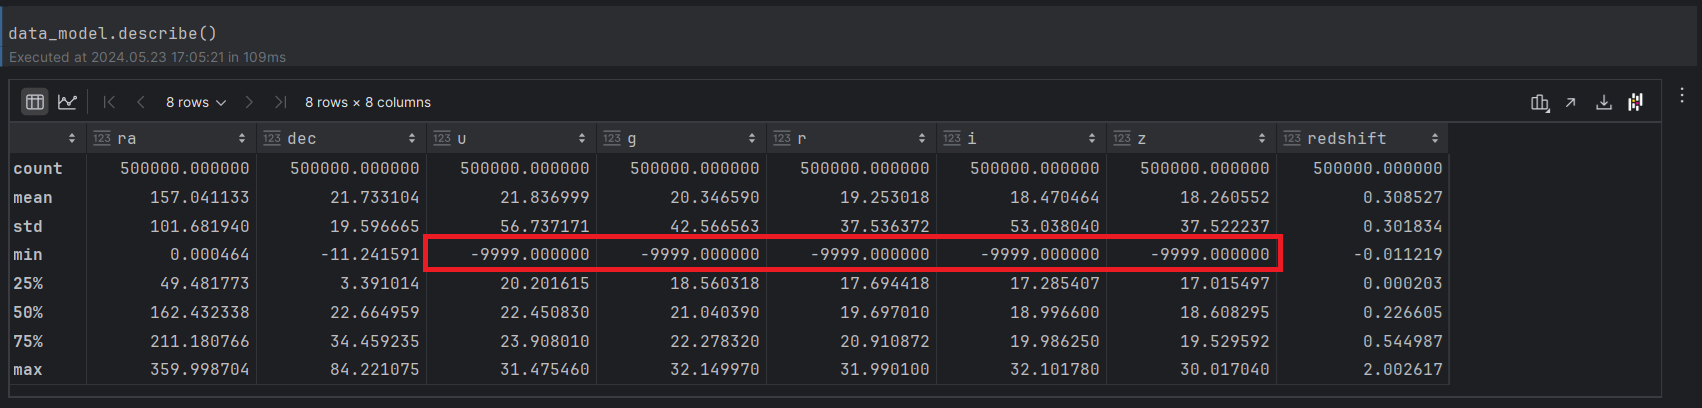
\includegraphics[width=0.8\textwidth]{data_model_anomalies.png}
\caption{Prikaz osnovne statistike skupa podataka}
\label{fig:sql_query}
\end{figure}

Na slici se vidi da određeni broj kolona koji se odnosi na magniture ima vrednost od -9999.00 što je predstavljalo placeholder za redove koje imaju grešku ili su nepoznate.\\\\
Koraci u procesu čišćenja podataka uključivali su:
\begin{itemize}
    \item \textbf{Provera atributa}: Prvo je provereno da li skup podataka sadrži kategoričke atribute. Pošto su svi atributi numerički, svi atributi su uključeni u primeni algoritma za detekciju outlier-a.
    \item \textbf{Filtriranje outlier-a}: Na osnovu rezultata LOF algoritma, podaci identifikovani kao outlier-i su uklonjeni iz skupa podataka.
\end{itemize}
Korišćenjem ovog pristupa, uspeli smo da identifikujemo i uklonimo outlier-e iz skupa podataka, čime smo poboljšali kvalitet podataka za treniranje modela. Nakon čišćenja podataka, preostalo je 492,153 redova koji su bili kvalitetni za dalju analizu.

\begin{figure}[h!]
\centering
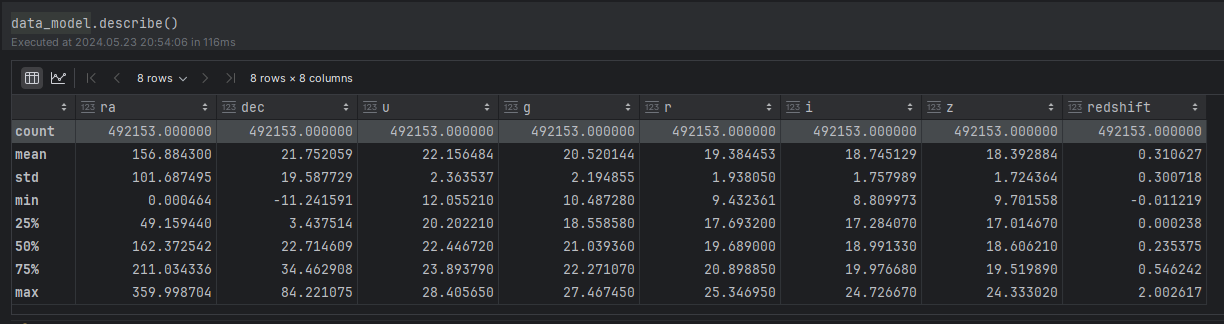
\includegraphics[width=0.8\textwidth]{data_model_filtered.png}
\caption{Skup podataka nakon uklanjanja outlier-a}
\label{fig:sql_query}
\end{figure}

\subsection{Odabrani atributi za treniranje modela}

Za treniranje klasifikacionih modela korišćeni su sledeći atributi: 'ra', 'dec', 'u', 'g', 'r', 'i', 'z', 'class', 'redshift', kao i izračunati atributi 'color\_u\_g', 'color\_g\_r', 'color\_r\_i', 'color\_i\_z'. Ovi atributi su pažljivo odabrani na osnovu njihove relevantnosti u astrofizici i njihove sposobnosti da pomognu u razlikovanju zvezda i galaksija.

\begin{itemize}
    \item \textbf{RA (Right Ascension)}: Ovo je jedna od dve osnovne nebeske koordinate koje se koriste za određivanje položaja nebeskih objekata na nebeskoj sferi. RA se meri u satima, minutima i sekundama, i predstavlja ugaonu udaljenost objekta istočno od Prolećne tačke. RA je ekvivalent geografskoj dužini na Zemlji.
    
    \item \textbf{DEC (Declination)}: Druga osnovna nebeska koordinata koja se koristi za određivanje položaja objekata na nebeskoj sferi. DEC se meri u stepenima, minutima i sekundama, i predstavlja ugaonu udaljenost objekta severno ili južno od nebeskog ekvatora. DEC je ekvivalent geografskoj širini na Zemlji.
    
    \item \textbf{Magnituda (u, g, r, i, z)}: Magnituda je mera sjaja nebeskog objekta viđenog sa Zemlje. Postoji pet filtera (u, g, r, i, z) koji mere sjaj u različitim delovima elektromagnetnog spektra:
    \begin{itemize}
        \item \textbf{u (ultraljubičasti filter)}: Mera sjaja u ultraljubičastom delu spektra.
        \item \textbf{g (zeleni filter)}: Mera sjaja u zelenom delu spektra.
        \item \textbf{r (crveni filter)}: Mera sjaja u crvenom delu spektra.
        \item \textbf{i (bliski infracrveni filter)}: Mera sjaja u bliskom infracrvenom delu spektra.
        \item \textbf{z (daleki infracrveni filter)}: Mera sjaja u dalekom infracrvenom delu spektra.
    \end{itemize}

        \item \textbf{Colour-indexes}: Ovi atributi su izračunati na osnovu magnituda i predstavljaju razliku između sjaja u različitim delovima spektra. Oni pružaju dodatne informacije o karakteristikama nebeskih objekata.
    \begin{itemize}
        \item \textbf{color\_u\_g}: Razlika između magnituda u ultraljubičastom (u) i zelenom (g) delu spektra: $color\_u\_g = u - g$.
        \item \textbf{color\_g\_r}: Razlika između magnituda u zelenom (g) i crvenom (r) delu spektra: $color\_g\_r = g - r$.
        \item \textbf{color\_r\_i}: Razlika između magnituda u crvenom (r) i bliskom infracrvenom (i) delu spektra: $color\_r\_i = r - i$.
        \item \textbf{color\_i\_z}: Razlika između magnituda u bliskom infracrvenom (i) i dalekom infracrvenom (z) delu spektra: $color\_i\_z = i - z$.
    \end{itemize}
    
    \item \textbf{Class (klasa)}: Ovaj atribut označava klasifikaciju objekta kao zvezda ili galaksija. Ovo je ciljna promenljiva u klasifikacionom modelu.
    
    \item \textbf{Redshift}: Crveni pomak je ključan fenomen u astronomiji jer omogućava određivanje udaljenosti i brzine udaljavanja nebeskih objekata, što je posebno važno za klasifikaciju između zvezda i galaksija. Razumevanje crvenog pomaka pomaže u identifikaciji galaksija koje se udaljavaju od nas zbog širenja svemira, dok zvezde, sa svojim karakterističnim relativnim brzinama unutar naše galaksije, pružaju dodatne informacije o njihovim kretanjima i položajima u odnosu na Sunčev sistem.
\end{itemize}

Atributi kao što su 'objid', 'run' i 'rerun' odnose se na administraciju podataka i nisu direktno bitni za izradu samog klasifikacionog modela. Atributi 'camcol', 'field', 'plate' i 'fiberid' predstavljaju tehničke podatke koji se odnose na uslove pod kojima je snimljen nebeski objekat. Atribut 'mjd' predstavlja modifikovani Julianov datum posmatranja i nije relevantan za određivanje da li je objekat zvezda ili galaksija.\\\\
Odabir ovih atributa omogućava modelima da imaju dovoljno informacija za preciznu klasifikaciju nebeskih objekata. RA i DEC pružaju informacije o položaju objekta na nebu, magnitude u različitim filterima omogućavaju analizu sjaja objekta u različitim delovima spektra, klasa objekta je cilj klasifikacije, dok crveni pomak pruža dodatne informacije o udaljenosti i brzini objekta.

\clearpage

\subsection{Vizualizacija podataka}

\subsubsection{Odnos broja instanci različitih klasa}
Prvo što želimo da uradimo, želimo da proverimo koji je odnos klasa koje imamo u našem skupu podataka.

\begin{figure}[h!]
\centering
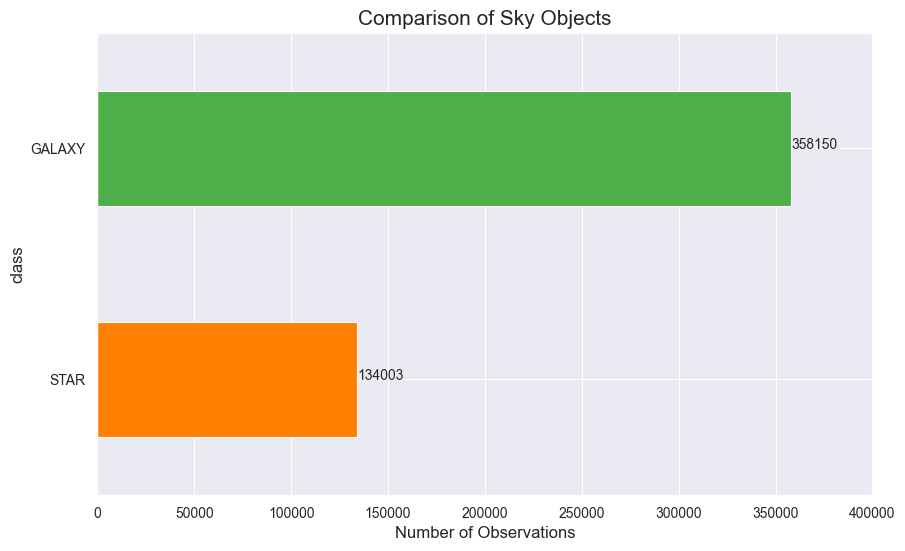
\includegraphics[width=0.8\textwidth]{class_count_result.png}
\caption{Odnos klasa u skupu podataka}
\label{fig:sql_query}
\end{figure}

Vidimo da u skupu podataka imamo mnogo veći broj galaksija u odnosu na broj zvezda, svakako model ćemo provobitno trenirati nad svim instancama.

\subsubsection{Prostorni raspored nebeskih tela}

\begin{figure}[h!]
\centering
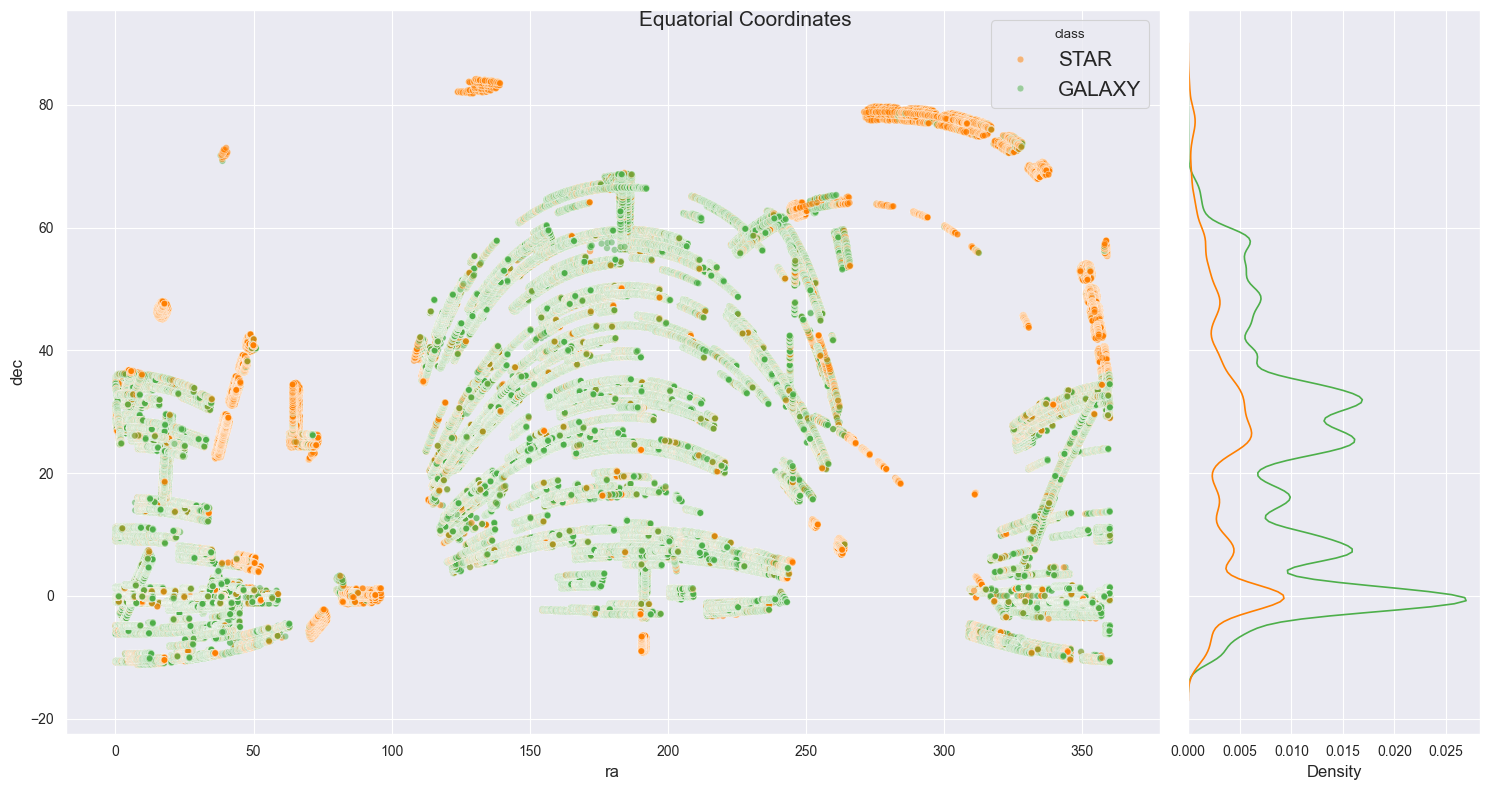
\includegraphics[width=0.8\textwidth]{equatorial_coordinate_map.png}
\caption{Prostorni raspored zvezda i galaksija u ekvatorijalnim koordinatama}
\label{fig:equatorial_coordinates}
\end{figure}

Sledeći grafikon prikazuje prostorni raspored zvezda i galaksija u ekvatorijalnim koordinatama. Iz grafikona se može videti da:

\begin{itemize}
    \item Zvezde (narandžaste tačke) su raspoređene u određenim regijama, često u skupovima, što ukazuje na oblasti sa visokom koncentracijom zvezda.
    \item Galaksije (zelene tačke) su takođe raspoređene u skupovima, ali pokazuju drugačiji obrazac rasporeda u odnosu na zvezde.
    \item Gustinski graf na desnoj strani pokazuje da postoji razlika u raspodeli zvezda i galaksija duž deklinacije, što može pomoći u daljem istraživanju i klasifikaciji objekata.
\end{itemize}

\subsubsection{Korelaciona matrica}

Korelaciona matrica je vizualni prikaz koji prikazuje međusobnu povezanost različitih atributa korišćenih u skupu podataka. Sledeći grafikon prikazuje korelacionu matricu za atribute zvezda i galaksija, omogućavajući nam da identifikujemo koje atribute imaju jaku ili slabu korelaciju.

\begin{figure}[h!]
\centering
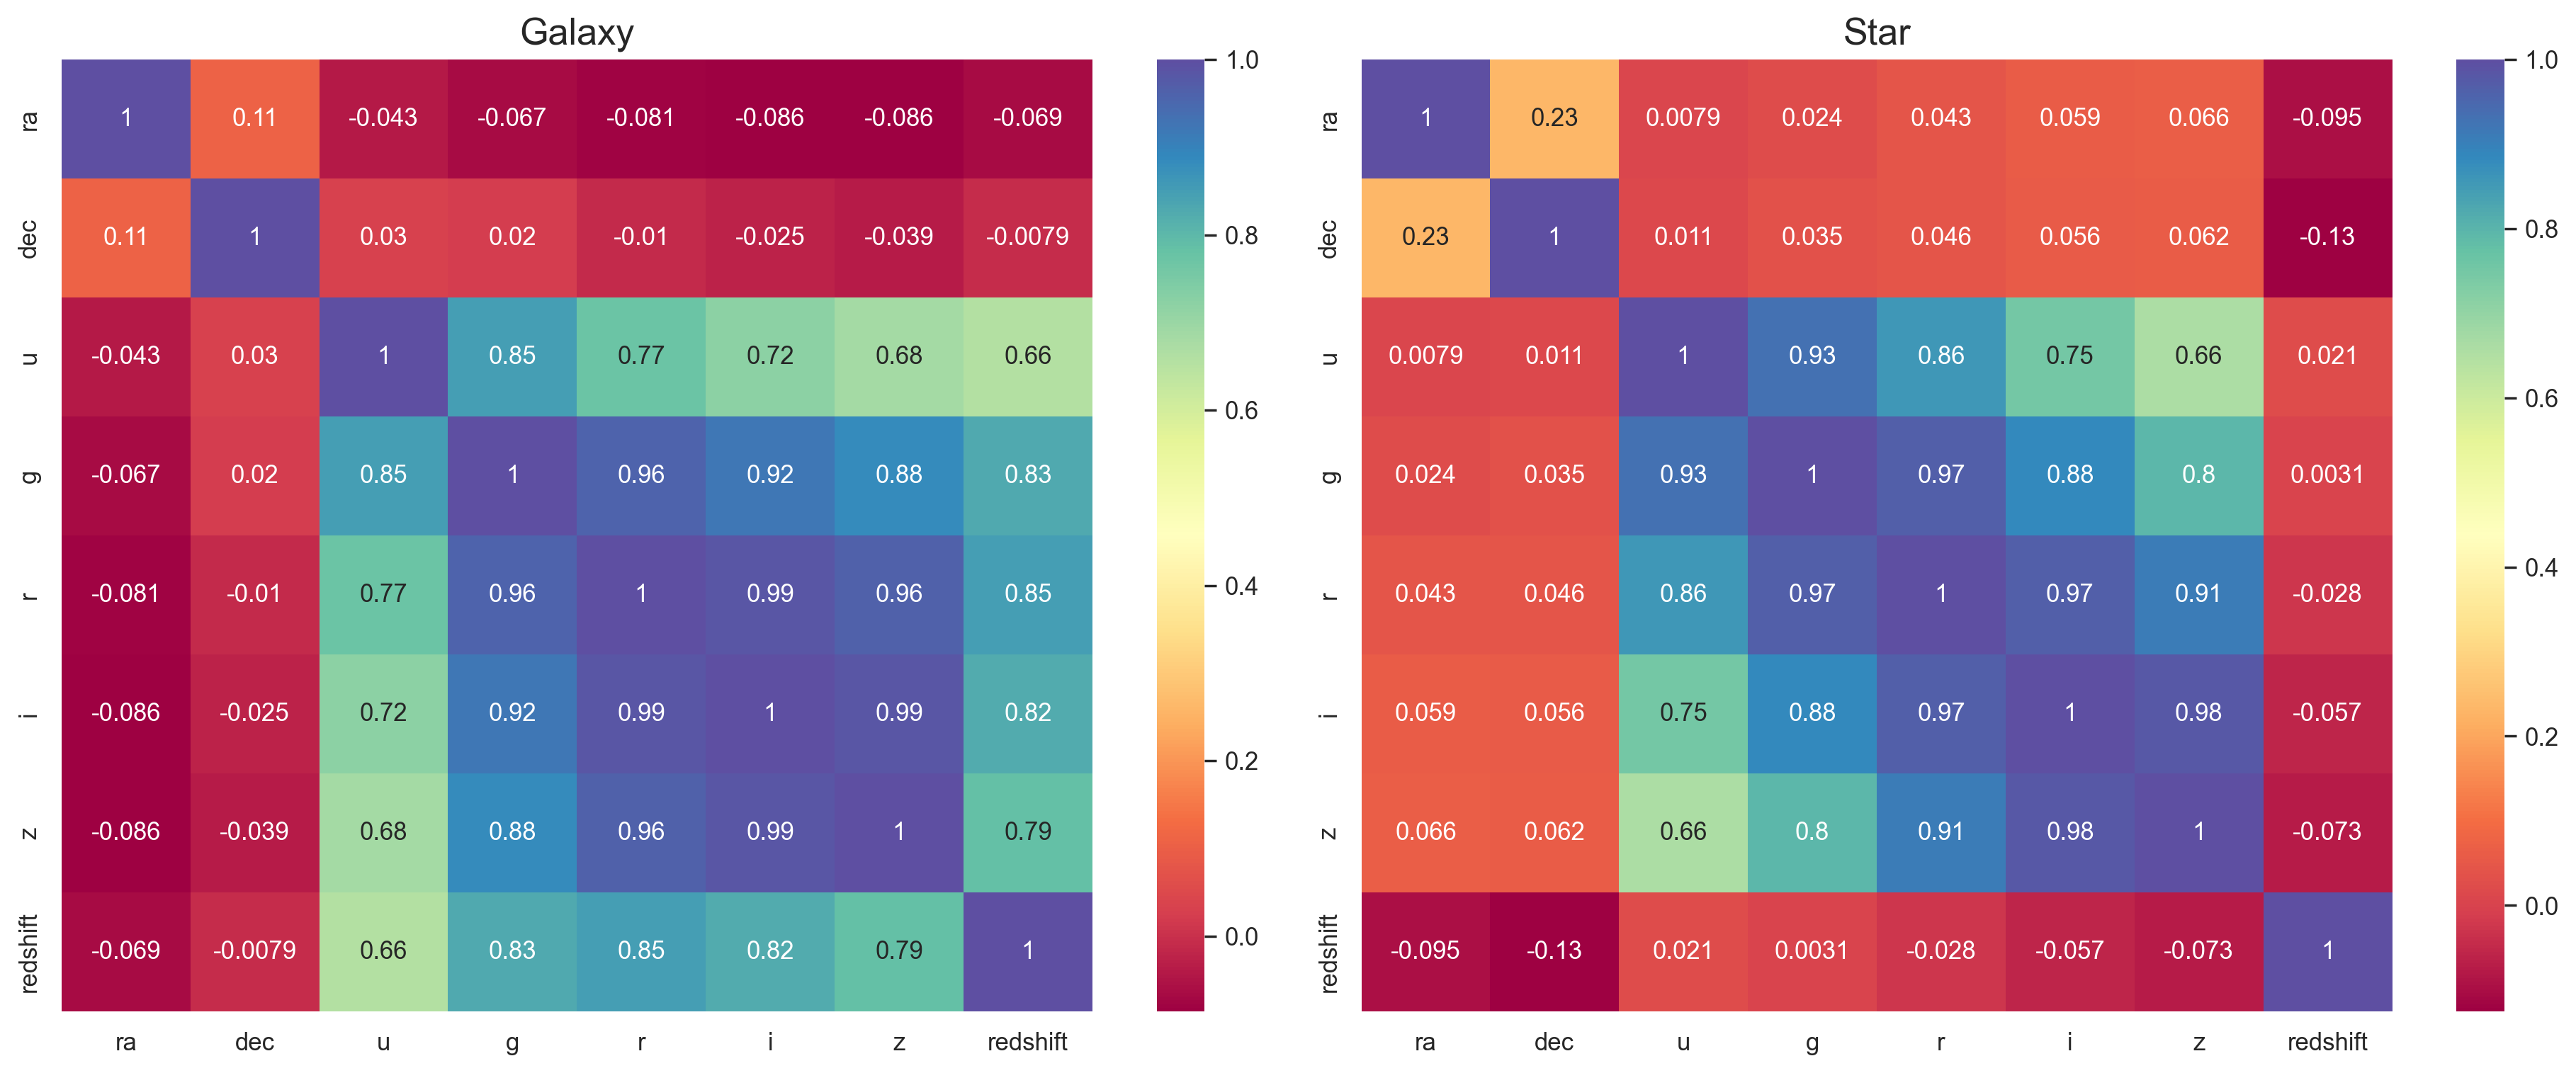
\includegraphics[width=0.8\textwidth]{correlation_matrix.png}
\caption{Korelaciona matrica za atribute zvezda i galaksija}
\label{fig:correlation_matrix}
\end{figure}

Na grafikonu su prikazane korelacije između atributa za zvezde (desno) i galaksije (levo).

\begin{itemize}
    \item \textbf{RA i DEC}: Vrednosti RA (Right Ascension) i DEC (Declination) imaju vrlo slabu korelaciju sa ostalim atributima. Ovo je očekivano jer su RA i DEC prostorne koordinate koje ne zavise direktno od fizičkih svojstava objekata kao što su magnitude i redshift.
    \item \textbf{Magnituda}: Magnitude u različitim filterima (u, g, r, i, z) pokazuju jaku pozitivnu korelaciju međusobno. Ovo znači da objekti koji su svetli u jednom filteru imaju tendenciju da budu svetli i u ostalim filterima.
    \item \textbf{Redshift}: Redshift pokazuje umereno pozitivnu korelaciju sa magnitudama. Ovo je logično jer objekti sa većim redshiftom (udaljeniji objekti) obično imaju drugačiji sjaj zbog kosmoloških efekata.
\end{itemize}

\subsection{Priprema podataka za treniranje modela}
Za uspešno treniranje i evaluaciju klasifikacionih modela, skup podataka je podeljen na tri dela: trening skup, validacioni skup i test skup. Ovaj pristup omogućava pravilnu procenu performansi modela i njegovu generalizaciju na nove podatke.

\subsubsection{Podela Skupa Podataka}
Skup podataka je podeljen na sledeći način:
\begin{itemize}
    \item \textbf{Trening Skup (Training Set)}: Ovaj skup podataka se koristi za treniranje modela. Model uči obrasce i veze između atributa na osnovu ovog skupa.
    \item \textbf{Validacioni Skup (Validation Set)}: Ovaj skup se koristi za validaciju modela tokom procesa treniranja. Validacioni skup omogućava podešavanje hiperparametara modela i sprečavanje preprilagođavanju modela. Ukoliko bismo izbacili ovaj skup, onda bismo evaluaciju modela radili na testnim podacima i ukoliko se ispostavi da su rezultati loši i da parametri algoritma moraju da se menjaju, značilo bi da model prilagođavamo testnim podacima koji bi trebali da ostanu "skriveni" sve do samog kraja.
    \item \textbf{Test Skup (Test Set)}: Ovaj skup se koristi za konačnu evaluaciju modela nakon što je treniran i validiran. Test skup pruža nezavisnu procenu performansi modela na novim, nepoznatim podacima.
\end{itemize}

Podaci su podeljeni tako da trening skup čini 60\% ukupnih podataka, validacioni skup 20\%, i test skup preostalih 20\%. Ova podela je odabrana kako bi se osiguralo da ima dovoljno podataka za treniranje modela, ali i dovoljno za validaciju i testiranje.\\
Takođe, prilikom podele podataka smo vodili pažnju da zadržimo originalni odnos zvezda i galaksija i u ovim podskupovima, kako ne bismo napravili trening i test skup koji su potencijalno još više disbalansirani.

\subsubsection{Skaliranje Podataka}
Skaliranje podataka je ključan korak u pripremi podataka za treniranje modela. Podaci su standardizovani tako da imaju srednju vrednost 0 i standardnu devijaciju 1. Ovo je važno jer određeni algoritmi klasifikacije zahtevaju skalirane podatke kako bi se izbeglo da atributi sa većim opsegom vrednosti postanu automatski važniji od ostalih atributa. Skaliranje osigurava da svi atributi imaju jednaku težinu prilikom treniranja modela.\\\\
Skaliranje podataka je takođe značajno za mnoge optimizacione algoritme, kao što je gradijentni spust, jer doprinosi bržoj konvergenciji i stabilnijem učenju modela. Standardizacija podataka omogućava algoritmima da efikasnije pretražuju prostor rešenja, što rezultira boljim performansama i bržim treniranjem.



\section{Klasifikacioni Algoritmi}

\subsection{Metrike za Evaluaciju Modela}
Za evaluaciju performansi klasifikacionih modela korišćene su sledeće metrike: tačnost (accuracy), preciznost (precision), odziv (recall), F1-score i podrška (support). Ove metrike omogućavaju sveobuhvatnu procenu kvaliteta modela i njegove sposobnosti da tačno klasifikuje nebeske objekte kao zvezde ili galaksije.\\
Važno je napomenuti da je skup podataka neuravnotežen, sa znatno većim brojem galaksija u odnosu na zvezde. U ovakvim situacijama, određene metrike, kao što su F1-score i odziv, postaju posebno važne za procenu performansi modela.

\begin{itemize}
    \item \textbf{Tačnost (Accuracy)}: Tačnost je mera koja pokazuje procenat tačno klasifikovanih instanci od ukupnog broja instanci. Visoka tačnost ukazuje na to da model dobro prepoznaje i zvezde i galaksije.
    \[
    \text{Tačnost} = \frac{\text{Broj tačno klasifikovanih instanci}}{\text{Ukupan broj instanci}}
    \]
    
    \item \textbf{Preciznost (Precision)}: Preciznost pokazuje koliko od svih instanci koje su modelom klasifikovane kao pozitivne (npr. zvezde) zaista pripada pozitivnoj klasi. Visoka preciznost znači da je mali broj lažno pozitivnih klasifikacija.
    \[
    \text{Preciznost} = \frac{\text{TP}}{\text{TP} + \text{FP}}
    \]
    gde su TP pravi pozitivni, a FP lažno pozitivni primerci.

    \item \textbf{Odziv (Recall)}: Odziv pokazuje koliko od svih stvarno pozitivnih instanci model tačno prepoznaje kao pozitivne. Visok odziv znači da je model sposoban da prepozna većinu pozitivnih instanci, što je posebno važno u neuravnoteženim datasetima gde je potrebno identifikovati što više pozitivnih instanci.
    \[
    \text{Odziv} = \frac{\text{TP}}{\text{TP} + \text{FN}}
    \]
    gde su TP pravi pozitivni, a FN lažno negativni primerci.

    \item \textbf{F1-score}: F1-score je harmonijska sredina preciznosti i odziva i koristi se kao jedinstvena mera performansi modela, naročito kada postoji neuravnoteženost klasa. F1-score uzima u obzir i preciznost i odziv, pružajući balansiranu meru performansi modela.
    \[
    \text{F1-score} = 2 \cdot \frac{\text{Preciznost} \cdot \text{Odziv}}{\text{Preciznost} + \text{Odziv}}
    \]

    \item \textbf{Podrška (Support)}: Podrška označava broj instanci u svakoj klasi u skupu podataka. Koristi se za procenu uravnoteženosti klasa i može uticati na izbor metrika za evaluaciju modela.
\end{itemize}

Uz ove metrike, koristili smo i matricu konfuzije za dodatnu evaluaciju modela. Matrica konfuzije je tabela koja prikazuje stvarne klase naspram predviđenih klasa, omogućavajući identifikaciju tačno i pogrešno klasifikovanih instanci. Redovi matrice predstavljaju stvarne klase, dok kolone predstavljaju predviđene klase. Matrica konfuzije pomaže u vizualizaciji performansi modela i identifikaciji specifičnih vrsta grešaka, kao što su lažno pozitivni i lažno negativni primerci.\\\\
Ove metrike omogućavaju sveobuhvatnu evaluaciju performansi modela, pružajući uvid u njegovu tačnost, sposobnost prepoznavanja pravih pozitivnih instanci i balans između preciznosti i odziva. U daljim sekcijama biće prikazani rezultati i obzervacije za svaki korišćeni algoritam.


\clearpage

\subsection{Stabla odlučivanja}
Decision tree (stablo odluke) je jedan od najjednostavnijih i najintuitivnijih algoritama za klasifikaciju. Radi tako što deli podatke na osnovu vrednosti atributa i pravi hijerarhijsku strukturu odluka, gde svaka grana predstavlja ishod odluke, a svaki čvor predstavlja atribut po kojem se podaci dele.


\subsubsection{Trening}

Za treniranje Decision Tree modela korišćen je skup podataka koji je prethodno podeljen na trening, validacioni i test skupove. Za treniranje modela nije bilo potrebno skalirati podatke, jer Decision Tree algoritmi ne zavise od udaljenosti između tačaka.

Decision Tree algoritmi imaju različite hiperparametre koji mogu uticati na kvalitet modela. Neki od tih hiperparametara uključuju maksimalnu dubinu stabla, minimalan broj uzoraka potrebnih za podelu čvora, minimalan broj uzoraka u listu i broj karakteristika koje se koriste za traženje najboljeg podele.

Kako bismo pronašli najbolju kombinaciju ovih hiperparametara, koristili smo GridSearchCV funkciju dostupnu u paketu sklearn, koja automatski pretražuje različite kombinacije hiperparametara i evaluira performanse modela za svaku od njih. Ovaj proces omogućava da se identifikuje konfiguracija hiperparametara koja daje najbolje rezultate za dati skup podataka. Takođe, jedan od parametara koji se prosleđuje ovoj funkciji predstavlja metriku koja će se koristiti za procenu kvaliteta modela prilikom pretrage, u ovom slučaju koristili smo f1 score s obzirom na neuravnoteženost podataka. Važno je napomenuti da se ove promene hiperparametara i traženje najboljeg modela zasnivaju na evaluaciji modela u svakoj iteraciji pretrage koristeći validacioni skup podataka.


\subsubsection{Rezultati}

Nakon optimizacije hiperparametara, Decision Tree model je evaluiran na test skupu podataka. Rezultati pokazuju visoku tačnost i odlične metrike za klasifikaciju.

\begin{figure}[h!]
\centering
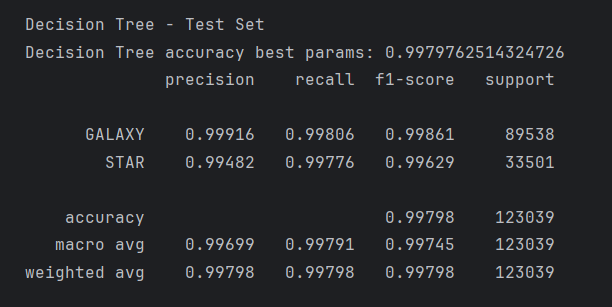
\includegraphics[width=0.8\textwidth]{decision_tree_classification_report.png}
\caption{Rezultati klasifikacije stabla odlučivanja na test skupu}
\label{fig:decision_tree_classification_report}
\end{figure}

Rezultati pokazuju da je model stabla odlučivanja vrlo efikasan u klasifikaciji nebeskih objekata, sa visokim vrednostima preciznosti, odziva i F1-score-a za obe klase.

\clearpage

Matrica konfuzije pruža dodatni uvid u rezultate evaluacije modela, prikazujući tačne i netačne klasifikacije za svaku klasu.

\begin{figure}[h!]
\centering
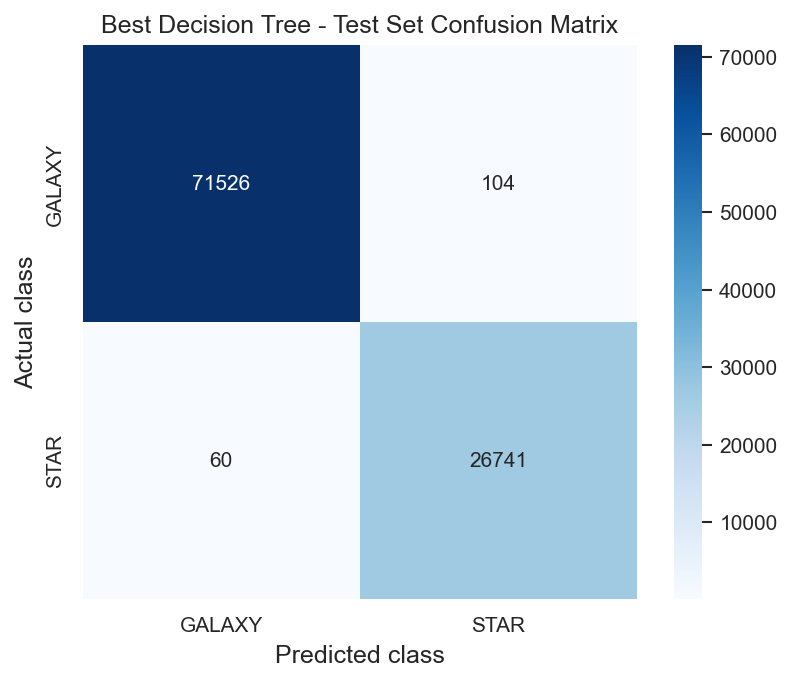
\includegraphics[width=0.6\textwidth]{decision_tree_cm.png}
\caption{Matrica konfuzije za model stabla odlučivanja na test skupu}
\label{fig:decision_tree_cm}
\end{figure}

Ovi rezultati potvrđuju da algoritam stabla odlučivanja može biti izuzetno efikasan za klasifikaciju nebeskih objekata, pružajući visok nivo tačnosti i pouzdanosti.

\subsection{Logistička regresija}
Logistička regresija (logistic regression) je popularan algoritam za binarnu klasifikaciju koji modelira verovatnoću da primerak pripada određenoj klasi. Algoritam koristi logističku funkciju za predikciju verovatnosti, a zatim klasifikuje primerke na osnovu praga verovatnoće (obično 0.5).

\subsubsection{Treniranje i evaluacija}
Za treniranje modela korišćen je skup podataka koji je prethodno podeljen na trening, validacioni i test skupove. Podaci su skalirani kako bi se obezbedila bolja konvergencija i kvalitet modela.

Kako bismo dodatno poboljšali kvalitet modela i smanjili varijansu, korišćena je unakrsna validacija. Ovaj pristup omogućava bolju procenu kvaliteta modela na različitim podskupovima podataka i pomaže u smanjenju uticaja neuravnoteženosti klasa.

\subsubsection{Rezultati Unakrsne Validacije}
Prosečna tačnost modela procenjena unakrsnom validacijom je pokazala visok nivo tačnosti, sa malim standardnim odstupanjem, što ukazuje na konzistentne performanse modela.

\begin{verbatim}
Mean Accuracy: 0.991 (0.001)
\end{verbatim}

\clearpage

\subsubsection{Rezultati}

\begin{figure}[h!]
\centering
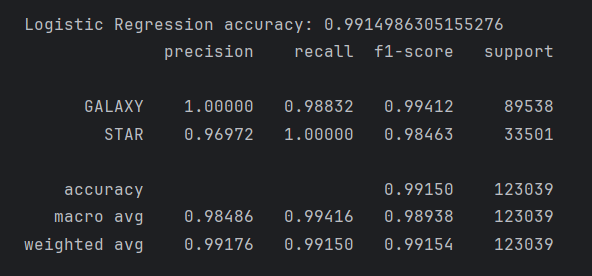
\includegraphics[width=0.8\textwidth]{logistic_regression_classification_report.png}
\caption{Rezultati klasifikacije modela na test skupu}
\label{fig:logistic_regression_classification_report}
\end{figure}

\begin{figure}[h!]
\centering
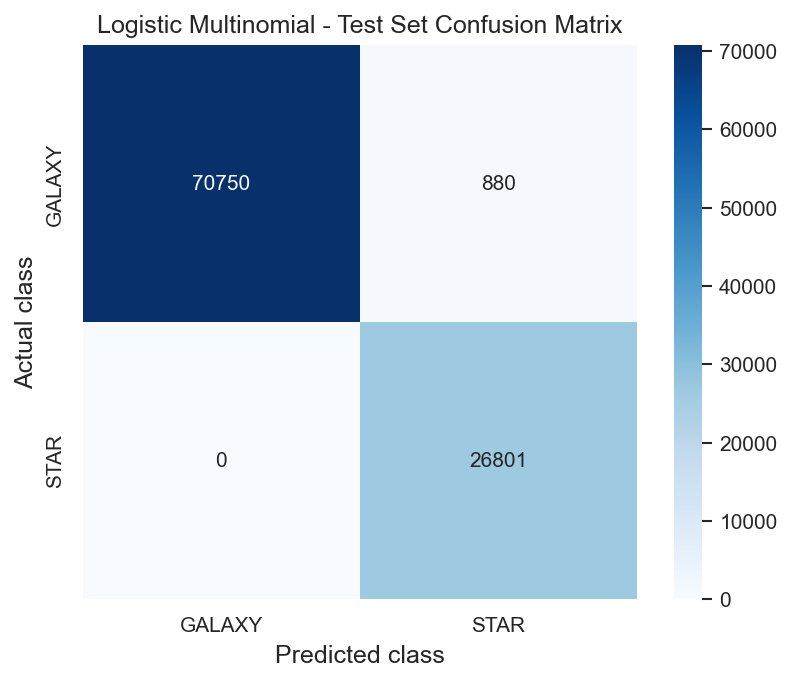
\includegraphics[width=0.6\textwidth]{logistic_regression_cm.png}
\caption{Matrica konfuzije za Logistic Regression model na test skupu}
\label{fig:logistic_regression_cm}
\end{figure}

Iako ovaj model postiže dobre sveobuhvatne metrike, kao što su visoka tačnost, preciznost i odziv, primećeno je da ima tendenciju grešaka u klasifikaciji galaksija. Konkretno, model često pogrešno klasifikuje galaksije kao zvezde, što je prikazano u matrici konfuzije na slici \ref{fig:logistic_regression_cm}.\\\\
Ova greška može biti značajna u određenim aplikacijama, čime stabla odlčivanja postaju bolji izbor za ovaj zadatak zbog veće preciznosti u razlikovanju klasa.

\subsection{K-najbližih suseda}

KNN(K-nearest neighbors= ili k-najbližih suseda je jednostavan, ali moćan algoritam mašinskog učenja koji se koristi za zadatke klasifikacije i regresije. U ovom slučaju mi ćemo ga koristiti za klasifikaciju. Klasifikacija najbližih suseda je deo opšte tehnike poznate kao učenje zasnovano na instancama, koja ne gradi globalni model, već koristi primere iz treniranja za pravljenje predikcija za test instance. (Stoga se za takve klasifikatore često kaže da su "bez modela.") Takvi algoritmi zahtevaju meru blizine kako bi odredili sličnost ili udaljenost između instanci i funkciju klasifikacije koja vraća predviđenu klasu test instance na osnovu njene blizine drugim instancama. Neke od mera udaljenosti koje se koristi za pronalaženje najbližeg suseda su: Euklidsko rastojanje, rastojanje Minkovskog, Hamingovo rastojanje, Menhetn rastojanje...

\subsubsection{Normalizacija i podela podataka}
Kao i kod svakog drugog modela mašinskog učenja potrebno je podeliti podatke na trening i test skupove. Kod k najbližih suseda neophodno je da su podaci normalizocani, zato što algoritam koristi meri udaljenost između tačaka.
Podatke treba normalizovati nakon što ih podelimo na trening i test skupove. Ovo je da bi se sprečilo "curenje podataka" jer bi normalizacija dala modelu dodatne informacije o test skupu ako bismo normalizovali sve podatke odjednom.

\subsubsection{Prilagođavanje i evaluacija modela}
Krećemo sa obučavanjem modela. Za ovo ćemo koristiti fiksiranu vrednost 5 za k, ali ćemo kasnije morati da optimizujemo ovo. Prvo kreiramo instancu KNN modela, zatim ćemo prilagoditi ovaj model našim trening podacima. Prosleđujemo i karakteristike i ciljnu promenljivu, tako da model može da uči.

Nakon što je model obučen. Možemo napraviti predikcije na test skupu podataka, koje kasnije možemo koristiti za ocenjivanje modela.
Najjednostavniji način za evaluaciju ovog modela je korišćenjem tačnosti. Proveravamo predikcije u odnosu na stvarne vrednosti u test setu i brojimo koliko je model tačno predvideo.
U našem slučaju to iznosi

\begin{verbatim}
    KNN accuracy - test set: 0.9829
\end{verbatim}

\subsubsection{Optimizacija algortima}
Izbor vrednosti 'k' igra ključnu ulogu u performansama KNN modela. Klasifikator sa malim brojem suseda odgovara visokoj složenosti modela što može dovesti do preprilagođavanja i verovatno će loše raditi na test skupu podataka. Sa druge strane, model sa mnogo suseda odgovara niskoj složenosti modela.
Unakrsna validacija je proces pri kojem se skup podataka nasumično deli na 'k' grupa. Jedna od grupa se koristi kao test skup, dok se ostale koriste kao trening skup. Model se trenira na trening skupu i ocenjuje na test skupu. Zatim se proces ponavlja dok svaka jedinstvena grupa ne bude korišćena kao test skup.

\begin{figure}[h!]
\centering
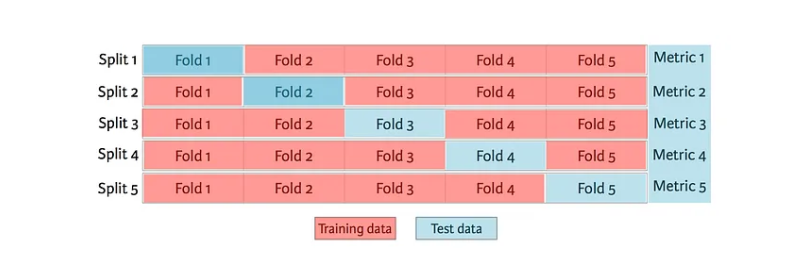
\includegraphics[width=0.6\textwidth]{cross-validation.png}
\caption{Unakrsna validacija}
\label{fig:cross_validation}
\end{figure}


GridSearchCV funkcioniše tako što trenira naš model više puta sa različitim parametrima koje smo naveli. Na taj način, možemo testirati naš model sa svakim parametrom i pronaći optimalne vrednosti kako bismo dobili najbolje rezultate tačnosti.

Prvo cemo odraditi grid pretragu da proverimo koji broj suseda ce dati najbolje performanse modela.
Nakon treniranja, možemo proveriti koji od naših testiranih vrednosti za n\textunderscore neighbors je najbolje performirao. Da bismo to uradili, pozvaćemo best\textunderscore params\textunderscore  na našem modelu.

\begin{verbatim}
    Best params:  {'n_neighbors': 6}
    Best estimator:  KNeighborsClassifier(n_neighbors=6)
    Best score:  0.9828044147934559
\end{verbatim}

Vizualizujmo sad performanse modela za različite vrednosti k na trening podacima. Najbolje performanse su koristeći oko 6 suseda. Što je broj suseda veći to model postaje jednostavniji i tačnost na trening skupu opada. Međutim, ako pogledate y-osu, razlika između tačnosti nije velika i bilo koja vrednost 'k' bi dobro obavila posao na našem problemu jer je najgora performansa oko 0.976.

\begin{figure}[h!]
\centering
\includegraphics[width=0.6\textwidth]{knn_accuracy_vs_k.png}
\caption{Odnos performansi modela i broja suseda}
\label{fig:knn_accuracy_vs_k}
\end{figure}

Kako bismo pobolj[ali model optimizujemo tri glavna hiperparametra koja utiču na prilagođavanje modela: n\textunderscore neighbours, weights i metric. Svi ostali hiperparametri ostaju na svojim podrazumevanim vrednostima.
\begin{verbatim}
    param_grid = {
        "n_neighbors": np.arange(1,12),
        "weights": ['uniform', 'distance'],
        "metric": ["euclidean","manhattan"],
        "n_jobs": [4]
    }
\end{verbatim}
\begin{itemize}
    \item n\textunderscore neighbors: Ovo predstavlja broj najbližih suseda koje k-NN algoritam treba da uzme u obzir.
    \item weights: Ovo određuje način na koji se računa doprinos svakog suseda. Postoje dve opcije:
    \begin{itemize}
        \item uniform: Svi susedi imaju isti doprinos bez obzira na udaljenost
        \item distance: Susedi bliži tački imaju veći doprinos nego udaljeni susedi.
    \end{itemize}
    \item metric: Ovo određuje način na koji se meri udaljenost između tačaka. Postoje dve opcije:
    \begin{itemize}
        \item euclidean
        \item manhattan
    \end{itemize}
    \item n\textunderscore jobs: Ovo određuje broj paralelnih zadataka koje treba pokrenuti prilikom obrade. Vrednost 4 znači da će se koristiti četiri procesorska jezgra za paralelnu obradu.

\end{itemize}
\subsubsection{Rezultati}
Rezultati su pokazali da je najbolja kombinacija parametara
\begin{verbatim}
Best params:  {'metric': 'manhattan', 'n_jobs': 4, 'n_neighbors': 6, 'weights': 'uniform'}
Best estimator:  KNeighborsClassifier(metric='manhattan', n_jobs=4, n_neighbors=6)
Best score:  0.9835416993884458
\end{verbatim}

Nakon što smo odradili optimizaciju modela vremem je da pokrenemo najbolje dobijen model na test podacima(podaci koje model nije jos uvek video) i da vidimo kolika će biti uspešnost modela.

\begin{figure}[h!]
\centering
\includegraphics[width=0.6\textwidth]{knn_best_est_result.png}
\caption{Rezultati KNN modela na test skupu}
\label{fig:knn_best_est_result}
\end{figure}

\begin{figure}[h!]
\centering
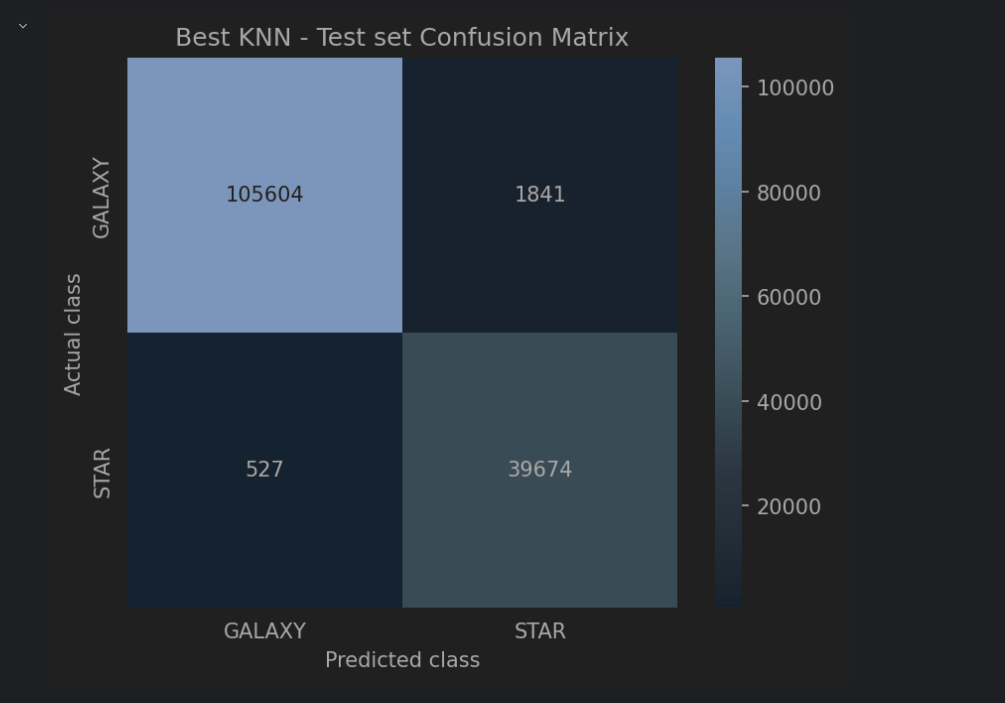
\includegraphics[width=0.6\textwidth]{knn_cm.png}
\caption{Matrica konfuzije za KNN model na test skupu}
\label{fig:knn_cm}
\end{figure}

Korišćenjem unakrsne validacije i grid pretrage možemo dobiti značajnije rezultate u poređenju sa našim originalnim deljenjem trening/test sa minimalnim podešavanjima. Unakrsna validacija je veoma važna metoda koja se koristi za kreiranje bolje prilagođenih modela obukom i testiranjem na svim delovima skupa podataka za obuku.
Iako unakrsna validacija može znatno koristiti razvoju modela, takođe postoji važna mana koja treba uzeti u obzir prilikom sprovođenja unakrsne validacije. Zbog toga što svaka iteracija modela, do k puta, zahteva da pokrenete ceo model, može postati računski skupo kako vaš skup podataka postaje veći i kako vrednost 'k' raste.

\section{Zaključak}


\begin{thebibliography}{9}
\bibitem{data_mining}
\end{thebibliography}

\end{document}
